\documentclass{ximera}

%\usepackage{todonotes}

\newcommand{\todo}{}

\usepackage{esint} % for \oiint
\ifxake%%https://math.meta.stackexchange.com/questions/9973/how-do-you-render-a-closed-surface-double-integral
\renewcommand{\oiint}{{\large\bigcirc}\kern-1.56em\iint}
\fi


\graphicspath{
  {./}
  {ximeraTutorial/}
  {basicPhilosophy/}
  {functionsOfSeveralVariables/}
  {normalVectors/}
  {lagrangeMultipliers/}
  {vectorFields/}
  {greensTheorem/}
  {shapeOfThingsToCome/}
  {dotProducts/}
  {partialDerivativesAndTheGradientVector/}
  {../productAndQuotientRules/exercises/}
  {../normalVectors/exercisesParametricPlots/}
  {../continuityOfFunctionsOfSeveralVariables/exercises/}
  {../partialDerivativesAndTheGradientVector/exercises/}
  {../directionalDerivativeAndChainRule/exercises/}
  {../commonCoordinates/exercisesCylindricalCoordinates/}
  {../commonCoordinates/exercisesSphericalCoordinates/}
  {../greensTheorem/exercisesCurlAndLineIntegrals/}
  {../greensTheorem/exercisesDivergenceAndLineIntegrals/}
  {../shapeOfThingsToCome/exercisesDivergenceTheorem/}
  {../greensTheorem/}
  {../shapeOfThingsToCome/}
  {../separableDifferentialEquations/exercises/}
}

\newcommand{\mooculus}{\textsf{\textbf{MOOC}\textnormal{\textsf{ULUS}}}}

\usepackage{tkz-euclide}\usepackage{tikz}
\usepackage{tikz-cd}
\usetikzlibrary{arrows}
\tikzset{>=stealth,commutative diagrams/.cd,
  arrow style=tikz,diagrams={>=stealth}} %% cool arrow head
\tikzset{shorten <>/.style={ shorten >=#1, shorten <=#1 } } %% allows shorter vectors

\usetikzlibrary{backgrounds} %% for boxes around graphs
\usetikzlibrary{shapes,positioning}  %% Clouds and stars
\usetikzlibrary{matrix} %% for matrix
\usepackage{pgfplots}
\usepgfplotslibrary{polar} %% for polar plots
\usepgfplotslibrary{fillbetween} %% to shade area between curves in TikZ
\usetkzobj{all}
\usepackage[makeroom]{cancel} %% for strike outs
%\usepackage{mathtools} %% for pretty underbrace % Breaks Ximera
%\usepackage{multicol}
\usepackage{pgffor} %% required for integral for loops



%% http://tex.stackexchange.com/questions/66490/drawing-a-tikz-arc-specifying-the-center
%% Draws beach ball
\tikzset{pics/carc/.style args={#1:#2:#3}{code={\draw[pic actions] (#1:#3) arc(#1:#2:#3);}}}



\usepackage{array}
\setlength{\extrarowheight}{+.1cm}
\newdimen\digitwidth
\settowidth\digitwidth{9}
\def\divrule#1#2{
\noalign{\moveright#1\digitwidth
\vbox{\hrule width#2\digitwidth}}}





\newcommand{\RR}{\mathbb R}
\newcommand{\R}{\mathbb R}
\newcommand{\N}{\mathbb N}
\newcommand{\Z}{\mathbb Z}

\newcommand{\sagemath}{\textsf{SageMath}}


%\renewcommand{\d}{\,d\!}
\renewcommand{\d}{\mathop{}\!d}
\newcommand{\dd}[2][]{\frac{\d #1}{\d #2}}
\newcommand{\pp}[2][]{\frac{\partial #1}{\partial #2}}
\renewcommand{\l}{\ell}
\newcommand{\ddx}{\frac{d}{\d x}}

\newcommand{\zeroOverZero}{\ensuremath{\boldsymbol{\tfrac{0}{0}}}}
\newcommand{\inftyOverInfty}{\ensuremath{\boldsymbol{\tfrac{\infty}{\infty}}}}
\newcommand{\zeroOverInfty}{\ensuremath{\boldsymbol{\tfrac{0}{\infty}}}}
\newcommand{\zeroTimesInfty}{\ensuremath{\small\boldsymbol{0\cdot \infty}}}
\newcommand{\inftyMinusInfty}{\ensuremath{\small\boldsymbol{\infty - \infty}}}
\newcommand{\oneToInfty}{\ensuremath{\boldsymbol{1^\infty}}}
\newcommand{\zeroToZero}{\ensuremath{\boldsymbol{0^0}}}
\newcommand{\inftyToZero}{\ensuremath{\boldsymbol{\infty^0}}}



\newcommand{\numOverZero}{\ensuremath{\boldsymbol{\tfrac{\#}{0}}}}
\newcommand{\dfn}{\textbf}
%\newcommand{\unit}{\,\mathrm}
\newcommand{\unit}{\mathop{}\!\mathrm}
\newcommand{\eval}[1]{\bigg[ #1 \bigg]}
\newcommand{\seq}[1]{\left( #1 \right)}
\renewcommand{\epsilon}{\varepsilon}
\renewcommand{\phi}{\varphi}


\renewcommand{\iff}{\Leftrightarrow}

\DeclareMathOperator{\arccot}{arccot}
\DeclareMathOperator{\arcsec}{arcsec}
\DeclareMathOperator{\arccsc}{arccsc}
\DeclareMathOperator{\si}{Si}
\DeclareMathOperator{\scal}{scal}
\DeclareMathOperator{\sign}{sign}


%% \newcommand{\tightoverset}[2]{% for arrow vec
%%   \mathop{#2}\limits^{\vbox to -.5ex{\kern-0.75ex\hbox{$#1$}\vss}}}
\newcommand{\arrowvec}[1]{{\overset{\rightharpoonup}{#1}}}
%\renewcommand{\vec}[1]{\arrowvec{\mathbf{#1}}}
\renewcommand{\vec}[1]{{\overset{\boldsymbol{\rightharpoonup}}{\mathbf{#1}}}}
\DeclareMathOperator{\proj}{\mathbf{proj}}
\newcommand{\veci}{{\boldsymbol{\hat{\imath}}}}
\newcommand{\vecj}{{\boldsymbol{\hat{\jmath}}}}
\newcommand{\veck}{{\boldsymbol{\hat{k}}}}
\newcommand{\vecl}{\vec{\boldsymbol{\l}}}
\newcommand{\uvec}[1]{\mathbf{\hat{#1}}}
\newcommand{\utan}{\mathbf{\hat{t}}}
\newcommand{\unormal}{\mathbf{\hat{n}}}
\newcommand{\ubinormal}{\mathbf{\hat{b}}}

\newcommand{\dotp}{\bullet}
\newcommand{\cross}{\boldsymbol\times}
\newcommand{\grad}{\boldsymbol\nabla}
\newcommand{\divergence}{\grad\dotp}
\newcommand{\curl}{\grad\cross}
%\DeclareMathOperator{\divergence}{divergence}
%\DeclareMathOperator{\curl}[1]{\grad\cross #1}
\newcommand{\lto}{\mathop{\longrightarrow\,}\limits}

\renewcommand{\bar}{\overline}

\colorlet{textColor}{black}
\colorlet{background}{white}
\colorlet{penColor}{blue!50!black} % Color of a curve in a plot
\colorlet{penColor2}{red!50!black}% Color of a curve in a plot
\colorlet{penColor3}{red!50!blue} % Color of a curve in a plot
\colorlet{penColor4}{green!50!black} % Color of a curve in a plot
\colorlet{penColor5}{orange!80!black} % Color of a curve in a plot
\colorlet{penColor6}{yellow!70!black} % Color of a curve in a plot
\colorlet{fill1}{penColor!20} % Color of fill in a plot
\colorlet{fill2}{penColor2!20} % Color of fill in a plot
\colorlet{fillp}{fill1} % Color of positive area
\colorlet{filln}{penColor2!20} % Color of negative area
\colorlet{fill3}{penColor3!20} % Fill
\colorlet{fill4}{penColor4!20} % Fill
\colorlet{fill5}{penColor5!20} % Fill
\colorlet{gridColor}{gray!50} % Color of grid in a plot

\newcommand{\surfaceColor}{violet}
\newcommand{\surfaceColorTwo}{redyellow}
\newcommand{\sliceColor}{greenyellow}




\pgfmathdeclarefunction{gauss}{2}{% gives gaussian
  \pgfmathparse{1/(#2*sqrt(2*pi))*exp(-((x-#1)^2)/(2*#2^2))}%
}


%%%%%%%%%%%%%
%% Vectors
%%%%%%%%%%%%%

%% Simple horiz vectors
\renewcommand{\vector}[1]{\left\langle #1\right\rangle}


%% %% Complex Horiz Vectors with angle brackets
%% \makeatletter
%% \renewcommand{\vector}[2][ , ]{\left\langle%
%%   \def\nextitem{\def\nextitem{#1}}%
%%   \@for \el:=#2\do{\nextitem\el}\right\rangle%
%% }
%% \makeatother

%% %% Vertical Vectors
%% \def\vector#1{\begin{bmatrix}\vecListA#1,,\end{bmatrix}}
%% \def\vecListA#1,{\if,#1,\else #1\cr \expandafter \vecListA \fi}

%%%%%%%%%%%%%
%% End of vectors
%%%%%%%%%%%%%

%\newcommand{\fullwidth}{}
%\newcommand{\normalwidth}{}



%% makes a snazzy t-chart for evaluating functions
%\newenvironment{tchart}{\rowcolors{2}{}{background!90!textColor}\array}{\endarray}

%%This is to help with formatting on future title pages.
\newenvironment{sectionOutcomes}{}{}



%% Flowchart stuff
%\tikzstyle{startstop} = [rectangle, rounded corners, minimum width=3cm, minimum height=1cm,text centered, draw=black]
%\tikzstyle{question} = [rectangle, minimum width=3cm, minimum height=1cm, text centered, draw=black]
%\tikzstyle{decision} = [trapezium, trapezium left angle=70, trapezium right angle=110, minimum width=3cm, minimum height=1cm, text centered, draw=black]
%\tikzstyle{question} = [rectangle, rounded corners, minimum width=3cm, minimum height=1cm,text centered, draw=black]
%\tikzstyle{process} = [rectangle, minimum width=3cm, minimum height=1cm, text centered, draw=black]
%\tikzstyle{decision} = [trapezium, trapezium left angle=70, trapezium right angle=110, minimum width=3cm, minimum height=1cm, text centered, draw=black]


\title[Dig-In:]{Approximating area with rectangles}

\outcome{Define area.}
\outcome{Understand the relationship between area under a curve and sums of rectangles.}
\outcome{Approximate area under a curve.}
\outcome{Compute left, right, and midpoint Riemann sums with 10 or fewer rectangles.}

\begin{document}
\begin{abstract}
  We introduce the basic idea of using rectangles to approximate the
  area under a curve.
\end{abstract}
\maketitle

\section{Rectangles and areas}

We want to compute the area between the curve $y=f(x)$ and the
horizontal axis on the interval $[a,b]$:

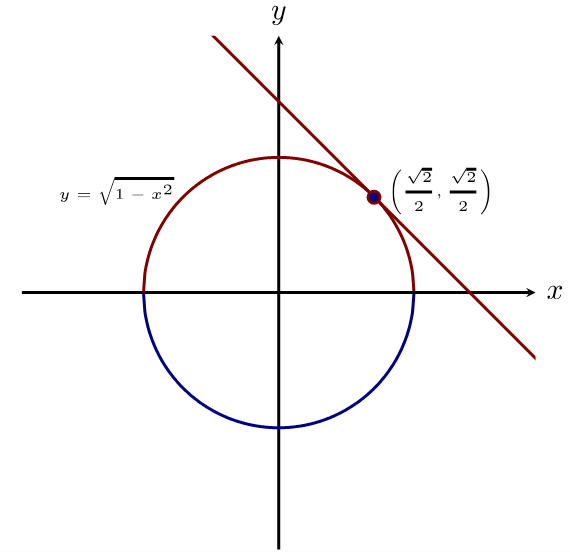
\includegraphics{0.png}

One way to do this would be to approximate the area with
rectangles. With one rectangle we get a rough approximation:
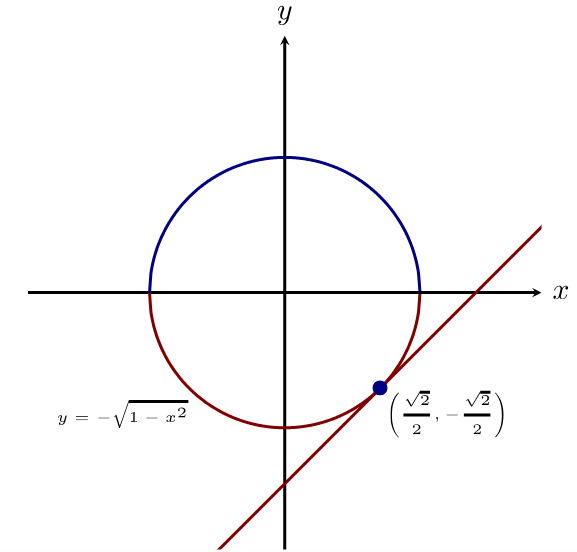
\includegraphics{1.png}
Two rectangles might make a better approximation:
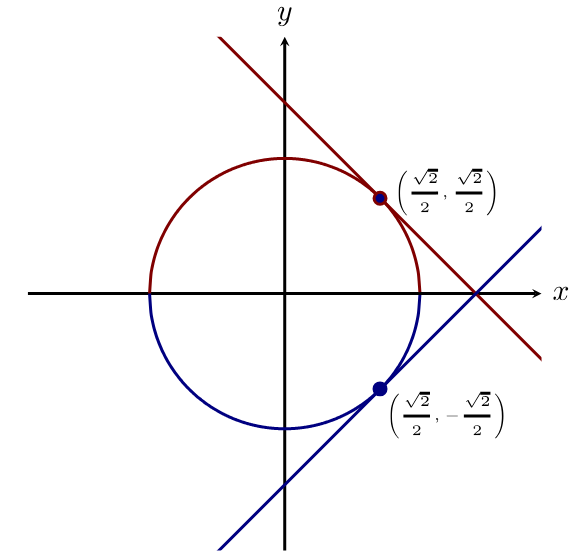
\includegraphics{2.png}
With even more, we get a closer, and closer, approximation:
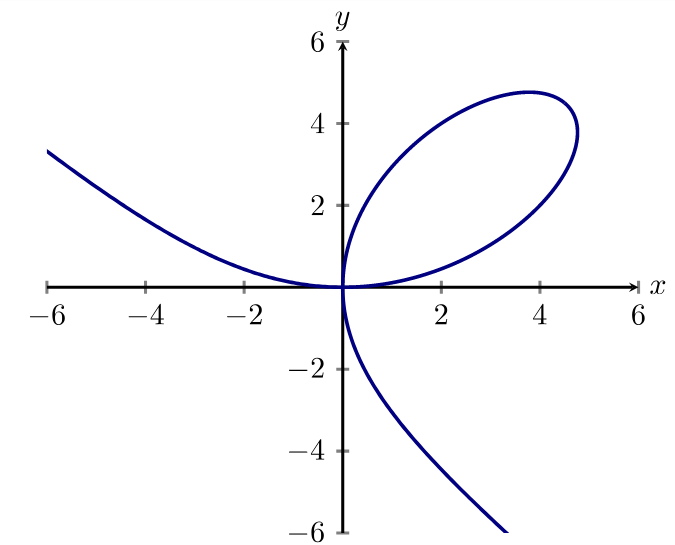
\includegraphics{3.png}

\begin{definition}
  If we are approximating the area between a curve and the $x$-axis
  on $[a,b]$ with $n$ rectangles of width $\Delta x$, then
  \[
  \Delta x = \frac{b-a}{n}.
  \]
\end{definition}
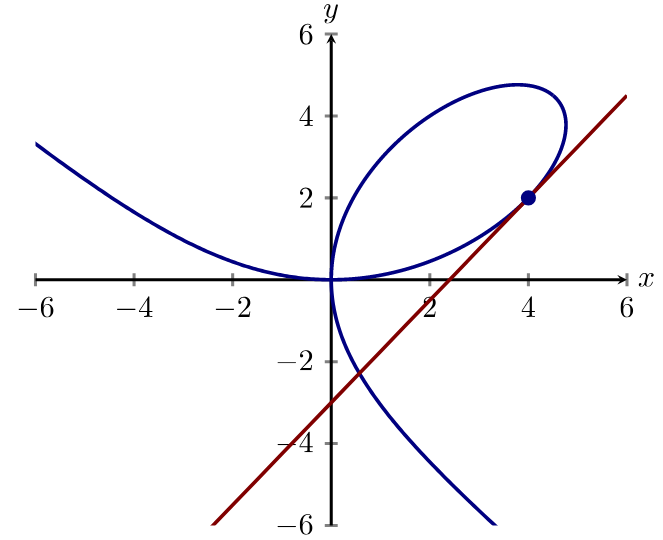
\includegraphics{4.png}
\begin{question}
  Suppose we wanted to approximate area between the curve $y=x^2+1$
  and the $x$-axis on the interval $[-1,1]$, with $8$ rectangles. What is $\Delta x$?
  \begin{prompt}
    \[
    \Delta x = \answer[given]{1/4}
    \]
  \end{prompt}
\end{question}

As we add rectangles, we are more closely approximating the area we are interested in:
\includegraphics{5.png}
We could find the area exactly if we could compute the limit as the
width of the rectangles goes to zero and the number of rectangles goes
to infinity.


Let's setup some notation to help with these calculations:


\begin{definition}
  When approximating an area with $n$ rectangles, the \dfn{grid
    points}
  \[
  x_0,x_1,x_2,\dots,x_n
  \]
  are the $x$-coordinates that determine the edges of the
  rectangles. In the graph below, we've numbered the rectangles to
  help you see the relation between the indices of the grid points
  and the $k$th rectangle.
\includegraphics{6.png}
Note, if we are approximating the area between a curve and the
horizontal axis on $[a,b]$ with $n$ rectangles, then it is always the
case that
\[
x_0=a\qquad\text{and}\qquad x_n = b.
\]
\end{definition}

\begin{question}
  If we are approximating the area between a curve and the horizontal
  axis with $11$ rectangles, how many grid points will we have?
  \begin{hint}
    You can draw it!
  \end{hint}
  \begin{prompt}
    We'll have $\answer[given]{12}$ grid points.
  \end{prompt}
\end{question}







\section{But which set of rectangles?}

When we use $n$ rectangles to
compute the area under a curve, the  width of each rectangle is $\Delta x=\frac{b-a}{n}$. It is clear that $\Delta x=x_k-x_{k-1}$, for $k=1,\dots, n$. 

But how do we determine 
\textit{the height} of the rectangle?

  We choose a \textit{sample point} $x_k^*$ and evaluate the function at that point. The value $f(x_k^*)$ determines the height of a rectangle.
\includegraphics{7.png}

\begin{definition}
  When approximating an area with rectangles, a \dfn{sample point} is
  the $x$-coordinate that determines the height of $k^{th}$
  rectangle. For  $k=1,\dots, n$, we denote a sample point as:
  \[
  x_k^*
  \]
  and the value
   \[
 f( x_k^*)
  \]
  is the height of the $k^{th}$ rectangle.
\end{definition}
\begin{question}
 What is the area of the $k^{th}$ rectangle shown in the figure above? 
  \begin{selectAll}
    \choice{$A=\Delta x $}
     \choice{$A=f(x)\Delta x $}
       \choice{$A= f( x_k^*)x_k^*$}
    \choice[correct]{$A= f( x_k^*)\Delta x$}
    \choice{$A=f(x)x$}  
     \choice{$A=k\Delta k$} 
       \choice[correct]{$A= f( x_k^*)(x_k-x_{k-1})$}
  \end{selectAll}
\end{question}
 Here
are three options for sample points that we consider:

\subsection{Rectangles defined by left-endpoints}

We can set the rectangles up so that the sample point is the left-endpoint.

\includegraphics{8.png}
In the graph above, the $k^{th}$ rectangle's left-endpoint determines the height of the rectangle.





\subsection{Rectangles defined by right-endpoints}

We can set the rectangles up so that the right-endpoint determines the height.

\includegraphics{9.png}
In the graph above, the $k^{th}$ rectangle's right-endpoint of the base determines the height.


\subsection{Rectangles defined by midpoints}

We can set the rectangles up so that the midpoint of the base determines the height.

\includegraphics{10.png}
In the graph above, the midpoint of the base of the $k^{th}$
rectangle determines the height.

%% \begin{question}
%%   Which approximation is most accurate?
%%   \begin{multipleChoice}
%%     \choice{Approximations with left-endpoints.}
%%     \choice{Approximations with right-endpoints.}
%%     \choice{Approximations with midpoints.}
%%     \choice[correct]{It depends on the function.}
%%   \end{multipleChoice}
%% \end{question}



\section{Riemann sums and approximating area}

Once we know how to identify our rectangles, we can compute approximations of some
 areas. If we are approximating area with $n$ rectangles, then 
\begin{align*}
  \text{Area} &\approx \sum_{k=1}^n (\text{height of $k$th rectangle})\times(\text{width of $k$th rectangle}) \\
  &=\sum_{k=1}^n  f(x_k^*)\Delta x \\
  &=  f(x_1^*)\Delta x +  f(x_2^*)\Delta x +   f(x_3^*)\Delta x + \dots +   f(x_n^*)\Delta x. 
\end{align*}


\begin{definition}
  A sum of the form:
  \[
  \sum_{k=1}^n  f(x_k^*)\Delta x  = f(x_1^*)\Delta x +  f(x_2^*)\Delta x + \dots +   f(x_n^*)\Delta x
  \]
  is called a \dfn{Riemann sum}, pronounced ``ree-mahn'' sum. 
\end{definition}

A Riemann sum computes an approximation of the area between a curve
and the $x$-axis on the interval $[a,b]$. It can be defined in several
different ways. In our class, it will be defined via left-endpoints,
right-endpoints, or midpoints. Here we see the explicit connection
between a Riemann sum defined by left-endpoints and the area between a curve
and the $x$-axis on the interval $[a,b]$:
\includegraphics{11.png}
and here is the associated Riemann sum
\[
\sum_{k=1}^5  f(x_k^*)\Delta x  = f(x_1^*)\Delta x +  f(x_2^*)\Delta x +   f(x_3^*)\Delta x + f(x_4^*)\Delta x + f(x_5^*)\Delta x.
\]



\subsection{Left Riemann sums}

\begin{example}
  Consider $f(x) = x^3/8-x+2$. Approximate the area between the curve $y=f(x)$ and
  the $x$-axis on the interval $[-1,3]$ using a \textbf{left-endpoint} Riemann
  sum with $n=5$ rectangles.
  
  \begin{explanation}
    First note that the width of each rectangle is
    \[
    \Delta x = \frac{3-(-1)}{5} = \answer[given]{4/5}.
    \]
    The grid points define the edges of the rectangle and are seen below:
\includegraphics{12.png}
On the other hand, the sample points identify which endpoints we use:
\includegraphics{13.png}
It is helpful to collect all of this data into a table:
\[
\begin{array}{c|c|c|c}
  k &  x_k & x^*_k & f(x^*_k) \\ \hline
  0 & \answer[given]{-1}   & \text{NA} & \text{NA}  \\
  1 & \answer[given]{-0.2} & \answer[given]{-1}        &   \answer[given]{2.875}     \\
  2 & \answer[given]{0.6}  & \answer[given]{-0.2}      & \answer[given]{2.199}   \\
  3 & \answer[given]{1.4}  & \answer[given]{0.6}       & \answer[given]{1.427}    \\
  4 & \answer[given]{2.2}  & \answer[given]{1.4}       & \answer[given]{0.943}   \\
  5 & \answer[given]{3}    & \answer[given]{2.2}      & \answer[given]{1.131}        \\
\end{array}
\]
Now we may write a left Riemann sum 
\[
f(x_1^*)\Delta x +  f(x_2^*)\Delta x +   f(x_3^*)\Delta x +f(x_4^*)\Delta x+   f(x_5^*)\Delta x,
\]
which evaluates to
\begin{align*}
  = 2.875 \cdot (4/5) &+ 2.199  \cdot(4/5) + 1.427  \cdot(4/5)\\
  &+ 0.943  \cdot(4/5) + 1.131  \cdot(4/5)
\end{align*}
and we find
\[
  = \answer[given]{6.86}.
\]
  \end{explanation}
\end{example}


\subsection{Right Riemann sums}


\begin{example}
  Consider $f(x) = x^3/8-x+2$. Approximate the area between the graph of $f$ and
  the $x$-axis on the interval $[-1,3]$ using a \textbf{right-endpoint} Riemann
  sum with $n=5$ rectangles.
  
  \begin{explanation}
    First note that the width of each rectangle is
    \[
    \Delta x = \frac{3-(-1)}{5} = \answer[given]{4/5}.
    \]
    The grid points define the edges of the rectangle and are seen below:
\includegraphics{14.png}
On the other hand, the sample points identify which endpoints we use:
\includegraphics{15.png}
It is helpful to collect all of this data into a table:
\[
\begin{array}{c|c|c|c}
  k &  x_k & x^*_k & f(x^*_k) \\ \hline
  0 & \answer[given]{-1}   & \text{NA} & \text{NA}  \\
  1 & \answer[given]{-0.2} & \answer[given]{-0.2}      & \answer[given]{2.199}   \\
  2 & \answer[given]{0.6}  & \answer[given]{0.6}       & \answer[given]{1.427}   \\
  3 & \answer[given]{1.4}  & \answer[given]{1.4}       & \answer[given]{0.943}   \\
  4 & \answer[given]{2.2}  & \answer[given]{2.2}       & \answer[given]{1.131}   \\
  5 & \answer[given]{3}    & \answer[given]{3}         & \answer[given]{2.375}   \\
\end{array}
\]
Now we may write a right Riemann sum 
\[
f(x_1^*)\Delta x +  f(x_2^*)\Delta x +   f(x_3^*)\Delta x +f(x_4^*)\Delta x+   f(x_5^*)\Delta x,
\]
which evaluates to
\begin{align*}
  = 2.199 \cdot (4/5) &+ 1.427  \cdot(4/5) + 0.943  \cdot(4/5)\\
  &+ 1.131  \cdot(4/5) + 2.375  \cdot(4/5)
\end{align*}
and we find
\[
  = \answer[given]{6.46}.
\]
  \end{explanation}
\end{example}




\subsection{Midpoint Riemann sums}

\begin{example}
  Consider $f(x) = x^3/8-x+2$. Approximate the area between the graph of $f$ and
  the $x$-axis on the interval $[-1,3]$ using a \textbf{midpoint }Riemann
  sum with $n=5$ rectangles.
  
  \begin{explanation}
    First note that the width of each rectangle is
    \[
    \Delta x = \frac{3-(-1)}{5} = \answer[given]{4/5}.
    \]
    The grid points define the edges of the rectangle and are seen below:
\includegraphics{16.png}
On the other hand, the sample points identify which endpoints we use:
\includegraphics{17.png}
It is helpful to collect all of this data into a table:
\[
\begin{array}{c|c|c|c}
  k &  x_k & x^*_k & f(x^*_k) \\ \hline
  0 & \answer[given]{-1}   & \text{NA} & \text{NA}  \\
  1 & \answer[given]{-0.2} & \answer[given]{-0.6}    & \answer[given]{2.573}   \\
  2 & \answer[given]{0.6}  & \answer[given]{0.2}     & \answer[given]{1.801}   \\
  3 & \answer[given]{1.4}  & \answer[given]{1}       & \answer[given]{1.125}   \\
  4 & \answer[given]{2.2}  & \answer[given]{1.8}     & \answer[given]{0.929}   \\
  5 & \answer[given]{3}    & \answer[given]{2.6}     & \answer[given]{1.597}   \\
\end{array}
\]
Now we may write a midpoint Riemann sum 
\[
f(x_1^*)\Delta x + f(x_2^*)\Delta x + f(x_3^*)\Delta x+ f(x_4^*)\Delta x + f(x_5^*)\Delta x,
\]
which evaluates to
\begin{align*}
  = 2.573 \cdot (4/5) &+ 1.801\cdot(4/5) + 1.125 \cdot(4/5) \\
  &+ 0.929 \cdot(4/5) + 1.597\cdot(4/5)
\end{align*}
and we find
\[
= \answer[given]{6.42}.
\]
  \end{explanation}
\end{example}

\begin{example}

Consider the function
\[
f(x) = 16 - x^2
\]
on the interval $[0,4]$. We will approximate the area between the graph of $f$ and the $x$-axis on the interval $[0,4]$. See the figure below.

\includegraphics{18.png}

The image depicts a \wordChoice{\choice{Left}\choice[correct]{Right}\choice{Midpoint}} Riemann sum with $n=\answer[given]{8}$ subintervals.

\begin{align*}
x_1^* &= \answer[given]{0.5}\\
f(x_1^*) &= \answer[given]{15.75}\\
x_6^* &= \answer[given]{3}\\
f(x_6^*) &= \answer[given]{7}\\
x_n^* &= \answer[given]{4}\\
f(x_n^*) &= \answer[given]{0}\\
\Delta x &= \answer[given]{\frac{1}{2}}\\
\sum_{k=1}^n f(x_k^*)\Delta x &= \answer[given]{38.5}
\end{align*}
This approximation is an \wordChoice{\choice{overestimate}\choice[correct]{underestimate}}. 
\end{example}

\begin{example}

Consider the function
\[
f(x) = 16 - x^2
\]
on the interval $[0,4]$. We will approximate the area between the graph of $f$ and the $x$-axis on the interval $[0,4]$ using a \textbf{right }Riemann
  sum with $n$ rectangles.
 First, determine the width of each rectangle.
  \[
  \Delta x = \answer[given]{\frac{4}{n}}\\
\]
Next, we will determine the grid-points.

\begin{align*}
x_0 &= \answer[given]{0}\\
 x_1 &=0+\Delta x=\frac{4}{n}\\
  x_2 &=  x_1+\Delta x=\answer[given]{2}\frac{4}{n}\\
   x_3 &= x_2+\Delta x= \answer[given]{3}\frac{4}{n}\\
   &\vdots\\
     x_{k-1}&= x_{k-2}+\Delta x=(\answer[given]{k-1})\frac{4}{n}\\
 x_k&= x_{k-1}+\Delta x=\answer[given]{k}\frac{4}{n}\\
 &\vdots\\
  x_n&=\answer[given]{4}.
\end{align*}
For a right Riemann sum, for $k=1,\dots,n$, we determine the sample points as follows:
\[
x_k^* = x_k=\answer[given]{k}\frac{4}{n}. 
\]
Now, we can approximate the area with a right Riemann sum.
\begin{align*}
  A\approx\sum_{k=1}^n  f(x_k^*)\Delta x  &= \sum_{k=1}^n  f(x_k)\frac{4}{n}  \\
  &= \sum_{k=1}^n  f\left(k\frac{4}{n}\right)\frac{4}{n}  \\
  &= \sum_{k=1}^n  \left(16-k^2\frac{16}{n^2}\right)\frac{4}{n}
\end{align*}
We can now simplify the last sum  by using the distribution, commutativity and associativity properties of a sum.
\begin{align*}
  A\approx \sum_{k=1}^n  \left(16-k^2\frac{16}{n^2}\right)\frac{4}{n} &=\frac{4}{n} \sum_{k=1}^n  \left(16-k^2\frac{16}{n^2}\right)\\
  &=\frac{4}{n}\left( \sum_{k=1}^n 16-\sum_{k=1}^n k^2\frac{16}{n^2}\right)
\end{align*}
In the last sum, the constant $\frac{16}{n^2}$ is a common factor, so we can again apply the distribution property and obtain the following 
\[
A\approx\frac{4}{n}\left( \sum_{k=1}^n 16-\frac{16}{n^2}\sum_{k=1}^n k^2\right)
\]
In the  first sum above, the constant $16$ is added $n$ times, and we have a formula for the second sum. Recall: $\sum_{k=1}^n k^2=\frac {n(n+1)(2n+1)}{6}$. Therefore,
\[
A\approx\frac{4}{n}\left(  n(16)-\frac{16}{n^2}\cdot\frac{n(n+1)(2n+1)}{6}\right)
\]
We can simplify this expression and obtain
\[
A\approx64-\frac{32(n+1)(2n+1)}{3n^2}
\]
This approximation is an \wordChoice{\choice{overestimate}\choice[correct]{underestimate}}. 

\begin{remark}
In our previous example we have computed a right Riemann sum for
$n=8$. Check whether your result was correct by plugging in $n=8$ in
the formula above.
\end{remark}
Now, we can take the limit of Riemann sums as  $n\to\infty$ to find the  exact value of the area of the region under the curve $y=f(x)$ on the interval $[0,4]$. Namely,  
\[
A=\lim_{n\to\infty}\sum_{k=1}^n  f(x_k^*)\Delta x, 
\]
and, therefore
\[
A=\lim_{n\to\infty}\left(64-\frac{32(n+1)(2n+1)}{3n^2}\right)=\answer[given]{\frac{128}{3}}.
\]
\end{example}


\subsection{Summary}

Riemann sums approximate the area between curves and the $x$-axis via
rectangles.  When computing this area via rectangles, there are
several things to know:
\begin{itemize}
\item What interval are we on? In our discussion above we call this
    $[a,b]$.
  \item How many rectangles will be used? In our discussion above we
    called this $n$.
  \item What is the width of each individual rectangle? In our discussion above we
    called this $\Delta x$.
  \item What points will determine the height of the rectangle? In our
    discussion above we called these sample points, $x_k^*$, and they
    can be left-endpoints, right-endpoints, or midpoints.
  \item What is the actual height of the rectangle? This will always
    be $f(x_k^*)$.
      \item We approximate the area $A$ with a Riemann sum
      
      $A\approx\sum_{k=1}^n  f(x_k^*)\Delta x$.
      \item As $n$ gets bigger and bigger,  $\Delta x$ gets smaller and smaller, and approximation gets better and better.
      We compute the exact value of $A$ by taking the limit of Riemann sums
      
      
     $A= \lim_{n\to\infty}\sum_{k=1}^n  f(x_k^*)\Delta x$.
\end{itemize}
\end{document}

